\begin{frame}{Python}
    \begin{columns}[c]        
        % Colonna Sinistra: Testo
        \begin{column}{0.48\textwidth}
        
        L'analisi è stata svolta in Python utilizzando le seguenti librerie:
        
        \begin{itemize}
        	\item ASE: gestione computazionale della struttura fisica
        	\item DScribe: test del metodo SOAP sui dati
        	\item Quippy: addestramento del potenziale
        \end{itemize}
        
        \end{column}
        % Colonna Destra: Due immagini incolonnate
        \begin{column}{0.24\textwidth}
        
            \centering
            
\includegraphics[scale=0.20]{./nobg/aselogo.png}
            
            \vspace{1.0em} % Spazio verticale tra le due immagini
            
            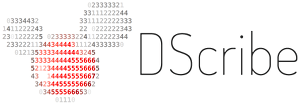
\includegraphics[scale=0.20]{./nobg/dscribelogo.png}
            
        \end{column}
        
        \begin{column}{0.24\textwidth}
        	
        	\centering
        	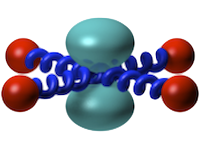
\includegraphics[scale=1.5]{./nobg/quippylogo.png}
        	
        	\vspace{0.8em} % Spazio verticale tra le due immagini
        	
        	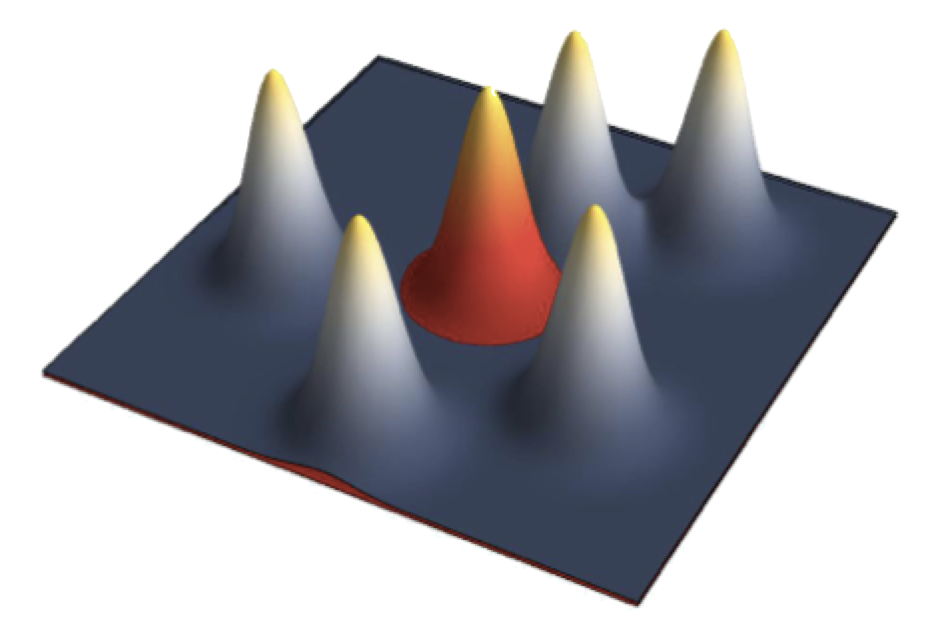
\includegraphics[scale=0.20]{./nobg/quippygaplogo.png}
        	
        \end{column}
        
    \end{columns}
\end{frame}


















